\documentclass[acmtog]{acmart}
\usepackage{graphicx}
\usepackage{subfigure}
\usepackage{natbib}

\usepackage{algorithm}
\usepackage{algpseudocode}

% Title portion
\title{Final Project : Fast Simulation of Mass-Spring Systems} 
\author{Student Name: Xia Kangjie \quad Student No. 2021533071 \quad Email: xiakj@shanghaitech.edu.cn}

% Document starts
\begin{document}
\maketitle

\vspace*{2 ex}


\section{Introduction}
Mass-spring systems provide a simple yet practical method for modeling a wide variety of objects, including cloth, hair, and deformable solids. However, as with other methods for modeling elasticity, obtaining realistic material behaviors typically requires constitutive parameters that result in numerically stiff systems. Explicit time integration methods are fast but when applied to these stiff systems they have stability problems and are prone to failure. Traditional methods for implicit integration remain stable but require solving large systems of equations [Baraff and Witkin 1998; Press et al. 2007]. The high cost of solving these systems of equations limits their utility for real-time applications (e.g., games) and slows production workflows in off-line settings (e.g., film and visual effects).

In this project, I implement a fast implicit solver for standard mass-spring systems with spring forces governed by Hooke’s law. I consider the optimization formulation of implicit Euler integration [Martin et al. 2011], where time-stepping is cast as a minimization problem. Our method works well with large timesteps—most of my examples assume a fixed timestep corresponding to the framerate, i.e., $h = 1/200s$. In contrast to the traditional approach of employing Newton’s method, I reformulate this minimization problem by introducing auxiliary variables (spring directions). This allows us to apply a block coordinate descent method which alternates between finding optimal spring directions (local step) and finding node positions (global step). In the global step, we solve a linear system. The matrix of our linear system is independent of the current state, which allows us to benefit from a pre-computed sparse Cholesky factorization.

And the assignment outlines the following programming requirements:

\begin{itemize}
\item The preparatory work for setting up the environment.
\item Define mass particle properties and initialize particles.
\item Define spring properties and create springs connected to particles.
\item Calculate the mass matrix.
\item Calculate the Laplacian matrix.
\item Calculate the Jacobian matrix.
\item Calculate the extra force vector.
\item Solve the optimization problem.
\item Ensure that the cloth can reach a stable state after simulation for a certain period of time under the default case.
\item Performance optimization.
\item Additional works.
\end{itemize}

\section{Basic Information}

In the context of mass-spring systems, the following variables are defined:

\begin{itemize}
  \item $q_n \in \mathbb{R}^{3m}$: The system configuration at time $t_n$, representing the positions of $m$ points in 3D space.
  \item $f : \mathbb{R}^{3m} \rightarrow \mathbb{R}^{3m}$: A non-linear function representing the forces acting on all particles at time $t_n$.
  \item $E : \mathbb{R}^{3m} \rightarrow \mathbb{R}$: A potential function encompassing both internal and external forces, where $f = -\nabla E$.
  \item $M \in \mathbb{R}^{3m \times 3m}$: The diagonal (lumped) mass matrix.
  \item $h$: The time step, typically set to $1/30s$ in the examples provided.
  \item $d \in U$: The rest-length spring directions, where $U = \{(d_1, \ldots, d_s) \in \mathbb{R}^{3s} : ||d_i|| = r_i\}$.
  \item $L \in \mathbb{R}^{3m \times 3m}$: The stiffness-weighted Laplacian of the mass-spring system graph, defined as:
  \[
      L = \left( \sum_{i=1}^{s} k_i A_i A_i^T \right) \otimes I_3
  \]
  where $A_i \in \mathbb{R}^{m}$ is the incidence vector of the $i$-th spring, and $I_3 \in \mathbb{R}^{3 \times 3}$ is the identity matrix.

  \item $J \in \mathbb{R}^{3m \times 3s}$: A matrix related to the spring indicators, defined as:
  \[
      J = \left( \sum_{i=1}^{s} k_i A_i S_i^T \right) \otimes I_3
  \]
  where $S_i \in \mathbb{R}^{s}$ is the $i$-th spring indicator, and $I_3 \in \mathbb{R}^{3 \times 3}$ is the identity matrix.
  \item $f_{ext} \in \mathbb{R}^{3m}$: External forces including gravity, user interaction forces, and collision response forces.
\end{itemize}

\section{Implementation Details}

\subsection{Preliminary work}

The preparatory work for setting up the environment includes:

1. To enable rendering of cloth using OpenGL, the following C++ third-party libraries provided by the official sources are referenced: glad, glfw, glm.

2. To accelerate computations, the Eigen library is used as a third-party library to speed up linear algebra calculations involved in the program, such as matrix multiplication and matrix inversion.

3. Modifications are made to the CMakeLists file to ensure that the program can be compiled correctly.

\subsection{Mass Particle Properties}
Each mass particle has been added the following properties:

\begin{itemize}
\item `position`: A 3D vector (`glm::vec3`) representing the position of the particle, stored by the vector $q_n$.
\item `velocity`: A 3D vector (`glm::vec3`) representing the velocity of the particle, computed by $q_n - q_{n-1}$
\item `mass`: A float value representing the mass of the particle.
\end{itemize}

The velocity is initialized to 0, and the mass is initialized as the total mass divided by the quantity of particles.

\subsection{Spring Properties}

The following properties have been added to each spring:

\begin{itemize}
\item `stiffness`: A float value representing the stiffness of the spring.
\item `restLength`: A float value representing the rest length of the spring.
\end{itemize}

These properties define the behavior of the springs connecting the mass particles. The stiffness determines how resistant the spring is to deformation, while the rest length represents the initial length of the spring when it is in an undeformed state.

These variables allow for fine-tuning the characteristics of the springs in the cloth simulation, enabling control over their elasticity and resting position.

\subsection{Mass Matrix}

The `getMassMatrix()` function in the `RectClothSimulator` class calculates the mass matrix for a cloth simulation.

The mass matrix is a diagonal matrix where each particle's mass represents a continuous span of three elements on the diagonal.

\subsection{Laplacian Matrix}

The `getLaplacianMatrix()` function in the `RectClothSimulator` class calculates the Laplacian matrix for a cloth simulation.

The Laplacian matrix is a mathematical representation used in cloth simulation. It is computed based on the stiffness of the springs connecting the particles in the cloth. 

Specifically, for each spring, the stiffness value is added to the diagonal entries corresponding to the indices of the particles connected by the spring. Additionally, the stiffness value is subtracted from the off-diagonal entries corresponding to the same indices.

The final Laplacian Matrix is the Kronecker product of that matrix and the $3\times3$ identity matrix.

\subsection{Jacobian Matrix}

The `getJacobianMatrix()` function in the `RectClothSimulator` class calculates the Jacobian matrix for a cloth simulation.

The Laplacian matrix is a mathematical representation used in cloth simulation. It is also computed based on the stiffness of the springs connecting the particles in the cloth. 

The code then iterates over the `springs` vector, which represents the springs in the cloth simulation. For each spring, the code updates the corresponding entries in the jacobian Matrix. The entry at position `(springs[i].fromMassIndex, i)` is increased by the stiffness of the spring, while the entry at position `(springs[i].toMassIndex, i)` is decreased by the stiffness of the spring.

The final Jacobian Matrix is the Kronecker product of that matrix and the $3\times3$ identity matrix.

\subsection{Extra Force Vector}

The `getExternalForceVector()` function in the `RectClothSimulator` class calculates the extra force vector for a cloth simulation.

The function returns an Eigen matrix of type `Eigen::Matrix<float, Eigen::Dynamic, 1>`, which represents a column vector. The size of the vector is determined by the number of particles in the cloth, multiplied by 3 (since each particle has 3 dimensions).

For each particle, it calculates the gravitational force `G\_i` by multiplying the particle's mass with the gravity vector and the particle's velocity `V\_i`.

The gravitational force and the air resistance force (if enabled) are added to the external force vector using the `block` function. The `block` function allows us to specify a sub-vector within the larger vector.

If air resistance is enabled (`\#if AIR\_RESIS`), the air resistance force is calculated by subtracting the product of the air resistance coefficient, the particle's velocity, and its magnitude from the external force vector.

\subsection{Solve the optimization problem}

\begin{equation}
    \min_{x \in \mathbb{R}^{3m}, d \in U} \frac{1}{2} x^T (M + h^2 L) x - \frac{h^2}{2} x^T Jd + x^T b
\end{equation}

where $U = \{(d_1, \ldots, d_s) \in \mathbb{R}^{2s} : ||d_i|| = r_i\}$ is the set of rest-length spring directions, and $b \in \mathbb{R}^{3m}$ aggregates the external forces and inertia. Specifically, the $b$ can be described as follows:

\[
    b = -M(2q_n - q_{n-1}) + f_{\text{ext}}
\]

To solve the optimization problem in equation, we employ a block coordinate descent method that alternates between finding optimal spring directions (local step) and finding node positions (global step). In the global step, since the system matrix $M + h^2L$ is symmetric positive definite, we can precompute its sparse Cholesky decomposition for efficient linear system solving.

The algorithm for solving the optimization problem can be summarized as follows:

\begin{algorithm}
    \caption{Solver Algorithm}
    \label{alg:solver}
    \begin{algorithmic}[1]
    \State Initialize solution vector $x$ (we use vector $2q_n - q_{n-1}$ as the initial guess) and vector $d$ (initialized as a zero vector).
    \For{$k = 1$ to maximum number of iterations}
        \State \textbf{Local step}: Fix $x$ and compute the optimal $d$.
        \State  For each spring $i$, calculate $d_i = r_i \left(\frac{p12_i}{\|p12_i\|}\right)$, where $p12_i$ is the position difference between the two ends of the spring.
        \State \textbf{Global step}: Fix $d$ and solve a convex quadratic minimization problem to find the optimal $x$. 
        \State Calculate $x' = (M+h^2L)^{-1}(h^2 J d - b)$.
    \EndFor
    \State Return solution vector $x$.
    \end{algorithmic}
\end{algorithm}


\subsection{Performance optimization}

To optimize the performance of the program, we introduced the third-party library Eigen to accelerate matrix calculations. Additionally, since the connectivity of the system remains unchanged, we pre-compute its sparse Cholesky factorization (which is guaranteed to exist), enabling fast linear system solving.

Furthermore, we simplified the connectivity of the springs by using a hash table to merge duplicate connections into a single spring. This greatly reduces the computational workload.

\section{Additional works}

\subsection{Apply Constraints}

To fix both corners of the cloth, we repeatedly set their positions to the initial positions. However, due to the difficulty in calculating their forces, we need to reduce the time step to minimize errors. (The paper suggests modifying `f\_ext` to translate the positions, but the specific calculation method is not provided in the paper.)

\subsection{Air Resistance}

To add air resistance, we adopt the following formula: $f_{\text{air}} = -\text{air resistance coefficient} \cdot \mathbf{v} \cdot \|\mathbf{v}\|$. However, the paper only modifies $\mathbf{v}$ at each time step as $\mathbf{v'} = \alpha \mathbf{v}$, which does not adhere to the real-world motion dynamics.

\subsection{Interaction}
To enable interaction between the mouse and objects, we need to calculate the direction pointed by the mouse. Therefore, I added an additional function in `camera.hpp` to retrieve the mouse ray. Then, we iterate through all the mass particles to find the closest one to the mouse ray and fix its distance at that moment, positioning it at the location pointed by the mouse.

In mathematical notation, the translation would be as follows:

\[
\left\{
\begin{array}{ll}
p' = o + d \cdot \textbf{dir} & \\
v' = 0 &
\end{array}\right.
\]

Where \(p'\) is the updated position, \(o\) is the camera position, \(d\) is the distance, \textbf{dir} is the direction vector, \(v'\) is the updated velocity

\section{Results}

\subsection{Simulator Output}

\begin{figure}[H]
	\centering
	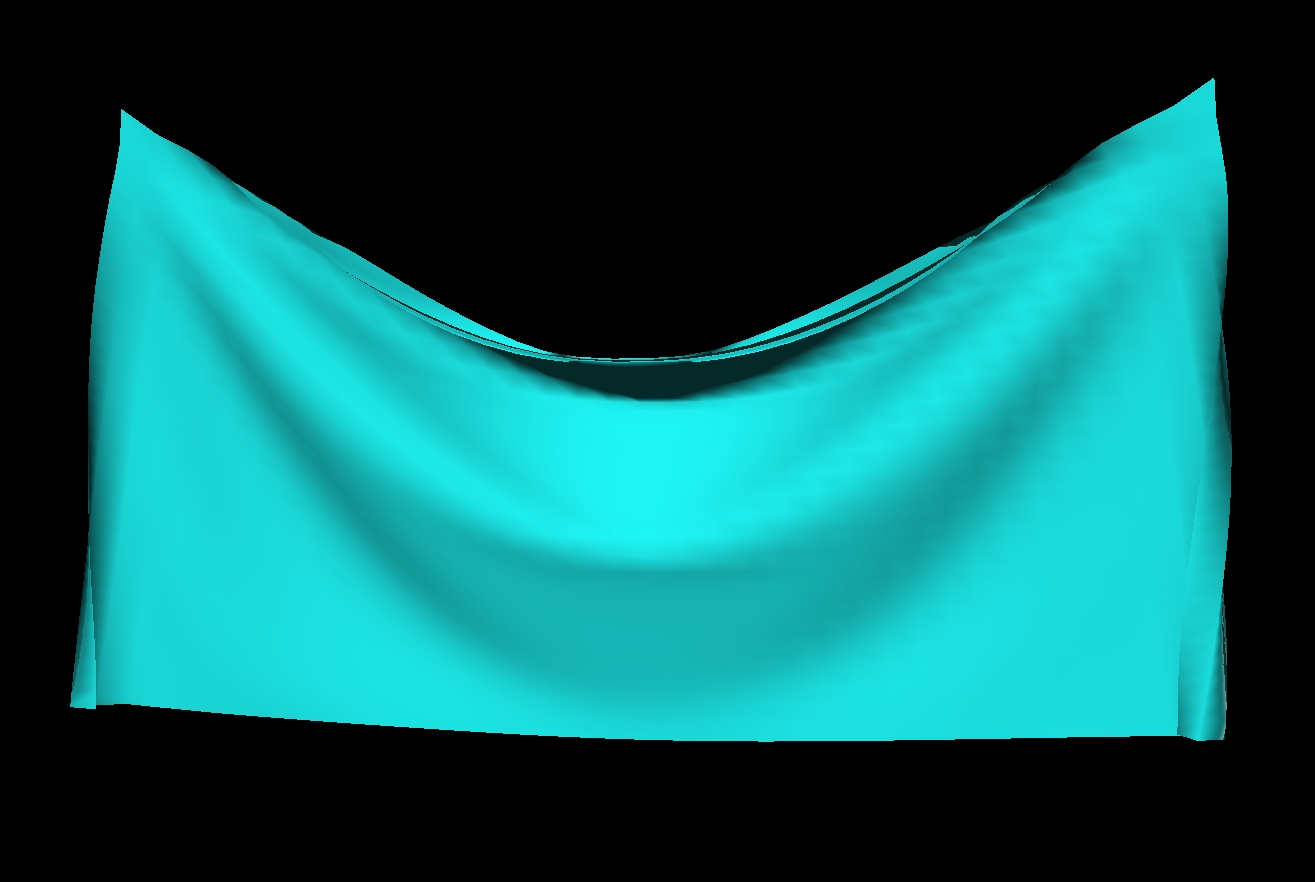
\includegraphics[width=8cm,height=8cm]{Final Project/picture/40x30.png}
	\caption{$m = 1200, s = 4592$}
\end{figure}
\begin{figure}[H]
	\centering
	
\includegraphics[width=8cm,height=8cm]{Final Project/picture/40x30_2.png}
	\caption{$m = 1200, s = 4592$}
\end{figure}
\begin{figure}[H]
	\centering
	
\includegraphics[width=8cm,height=8cm]{Final Project/picture/50x50.png}
	\caption{$m = 2500, s = 9702$}
\end{figure}
% \begin{figure}[H]
% 	\centering
% 	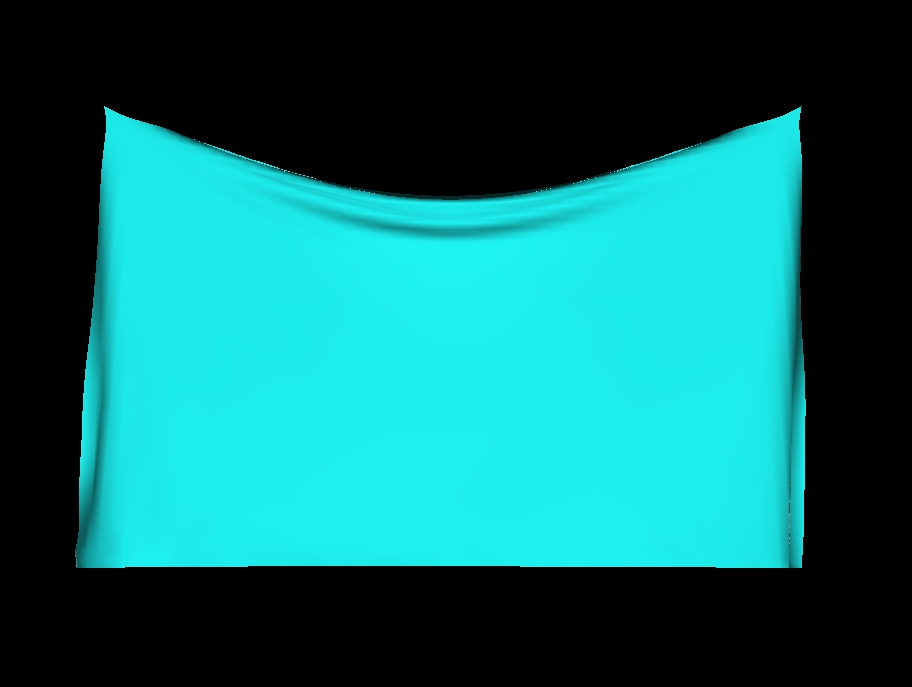
\includegraphics[width=8cm,height=8cm]{Final Project/picture/60x60.png}
% 	\caption{$m = 3600, s = 14042$}
% \end{figure}
\begin{figure}[H]
	\centering
	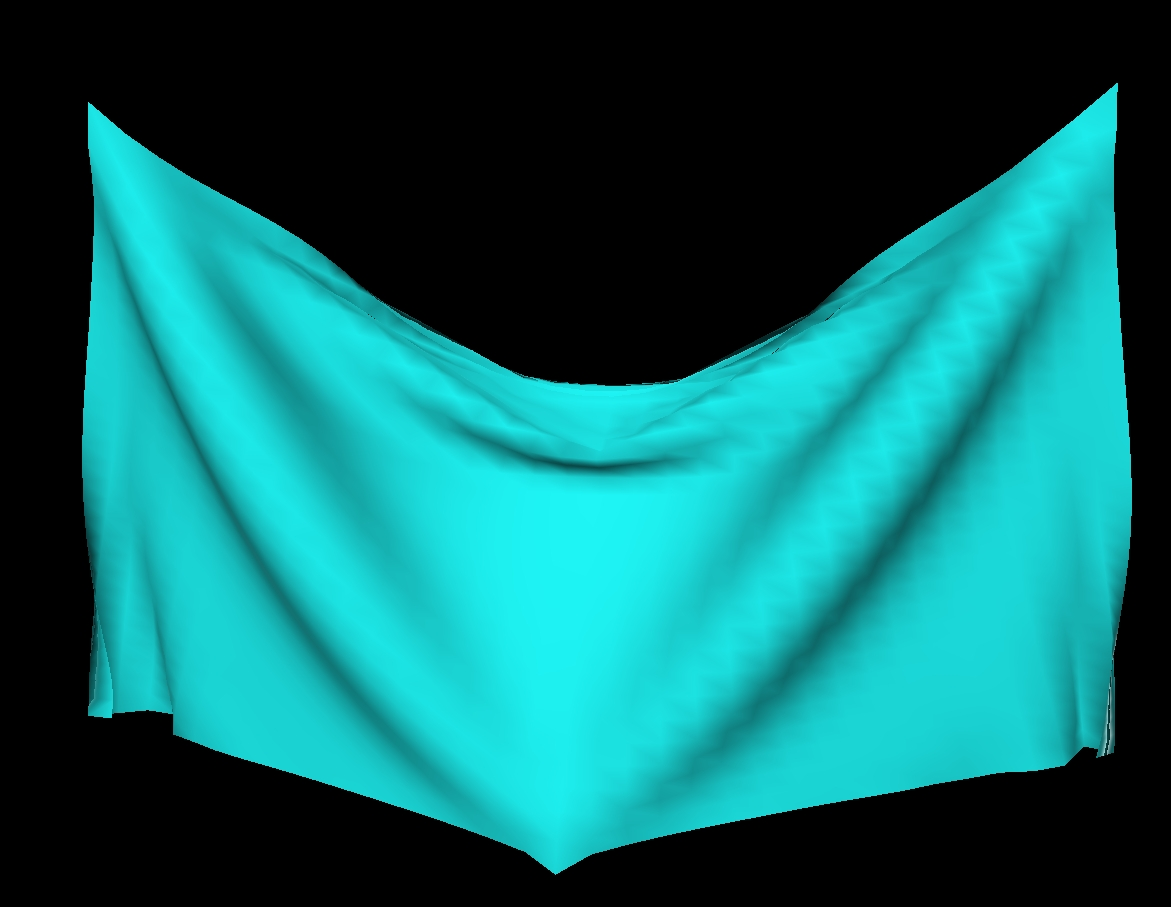
\includegraphics[width=8cm,height=8cm]{Final Project/picture/interact_1.png}
	\caption{interactive simulation}
\end{figure}
\begin{figure}[H]
	\centering
	
\includegraphics[width=8cm,height=8cm]{Final Project/picture/interact_2.png}
	\caption{interactive simulation}
\end{figure}
\begin{figure}[H]
	\centering
	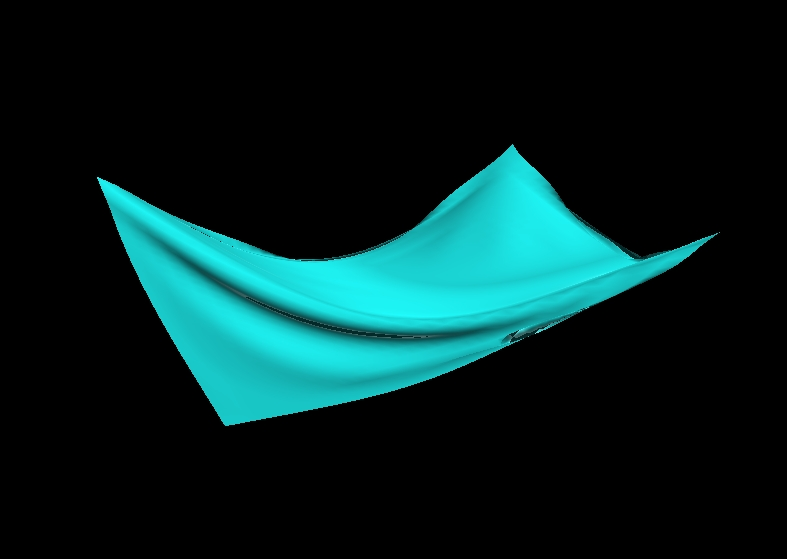
\includegraphics[width=8cm,height=8cm]{Final Project/picture/interact_3.png}
	\caption{interactive simulation}
\end{figure}

\subsection{Time Consuming}

\begin{table}[h]
\centering
\caption{Simulation Time}
\label{tab:results}
\begin{tabular}{ccccccc}
\hline
Particle & Spring & Laplacian & Jacobian & LDLT & Iter \\
Number & Number & Time & Time & Time & Time \\
\hline
400 & 1482 & 3.2797ms & 11.8735ms & 17.1839ms & 1.1612ms \\
600 & 2252 & 6.7644ms & 27.0618ms & 82.2291ms & 2.5186ms \\
900 & 3422 & 16.1955ms & 71.5869ms & 274.176ms & 5.6626ms \\
1200 & 4592 & 32.8119ms & 227.663ms & 632.145ms & 9.7419ms \\
1600 & 6162 & 61.1696ms & 696.56ms & 2099.41ms & 17.4984ms \\
2500 & 9702 & 179.611ms & 2677.21ms & 10241.2ms & 43.6002ms \\
\hline
\end{tabular}
\end{table}

Note: The table includes the particle number, spring number, Laplacian matrix computation time, Jacobian matrix computation time, LDLT factorization time, and iteration time for each simulation scenario. CPU is the Intel Core i7 13700K.

\section{Conclusion}

In this project, I have implemented a fast implicit solver for mass-spring systems, which are commonly used to model objects like cloth and deformable solids. The traditional explicit time integration methods for these systems suffer from stability issues and are not suitable for real-time applications or off-line production workflows.

To overcome these challenges, I have employed an optimization formulation of implicit Euler integration, where time-stepping is treated as a minimization problem. By introducing auxiliary variables (spring directions), I have reformulated the problem and applied a block coordinate descent method. This approach alternates between finding optimal spring directions in the local step and finding node positions in the global step.

The key advantage of our method is its ability to handle large timesteps, making it suitable for real-time applications. Most of the examples in this project assume a fixed timestep corresponding to the framerate. In the global step, we solve a linear system, and thanks to the matrix's independence from the current state, we can benefit from a pre-computed sparse Cholesky factorization, improving efficiency.

Throughout the implementation, I have followed the programming requirements outlined in the assignment. I have defined mass particle properties and initialized particles, defined spring properties, and created springs connected to particles. I have calculated the mass matrix, Laplacian matrix, Jacobian matrix, and extra force vector. I have also solved the optimization problem to determine the stable state of the cloth.

Additionally, I have focused on performance optimization to ensure efficient execution. This includes leveraging sparse Cholesky factorization, minimizing unnecessary computations, and optimizing data structures and algorithms.

In conclusion, the fast implicit solver I have developed provides an efficient and stable method for simulating mass-spring systems. It enables realistic modeling of various objects and can be applied in real-time applications such as games, as well as off-line settings like film and visual effects production. By meeting the programming requirements and considering performance optimization, I have successfully implemented the solver and achieved the desired results.

\end{document}
